\begin{surferPage}[Double Cone]{A Double Cone}
   As explained in the introduction to this gallery a surface is called
    \emph{non--singular} or smooth if it does not have any apexes
    (such points are called singularities).
    For example, a sphere or a torus (two leftmost pictures below):
    \begin{center}
      \begin{tabular}{@{}c@{}c@{}c@{}c@{}}
        \begin{tabular}{@{}c}
          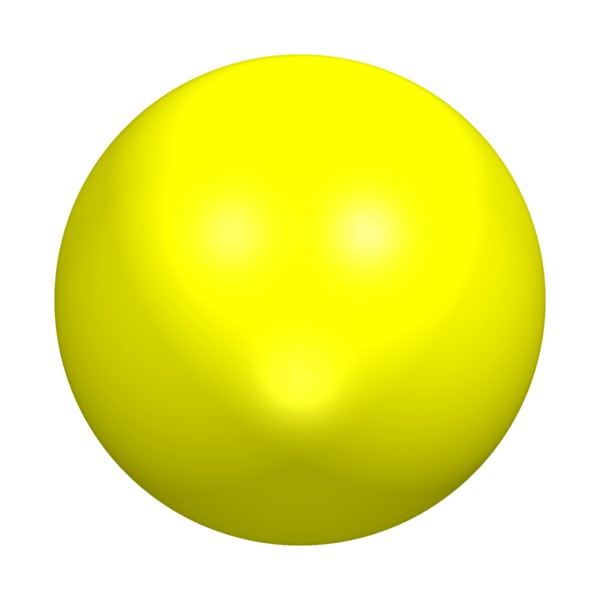
\includegraphics[width=1.4cm]{./../../common/images/kugel}
        \end{tabular}
        &
        \begin{tabular}{@{}c}
          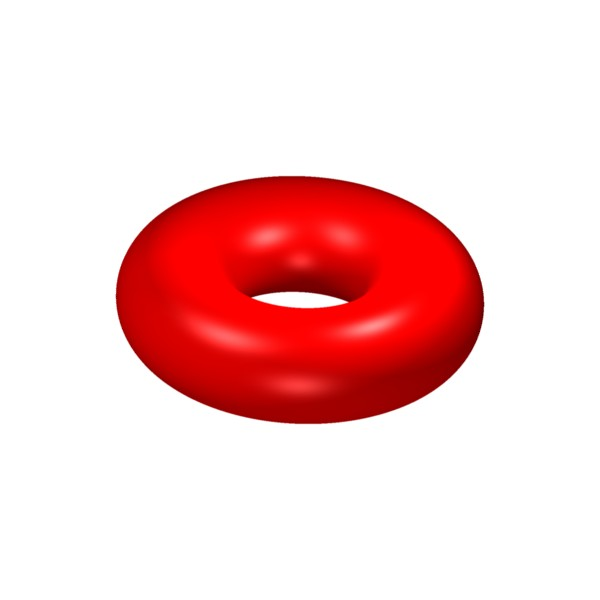
\includegraphics[width=1.4cm]{./../../common/images/torus}
        \end{tabular}
        &
        \begin{tabular}{c@{}}
          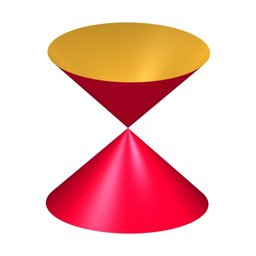
\includegraphics[width=1.4cm]{./../../common/images/kegel}
        \end{tabular}
      \end{tabular}
    \end{center}
     The double cone (rightmost picture) is the simplest singularity; it is the only singularity which can be described by an equation of
    degree $2$:
    \[x^2+y^2-z^2=0.\]
    When changing this equation slightly by replacing the $0$ with a small value
    $a\neq 0$, the double cone transforms into one of the two types of
    hyperboloids, depending on the sign of $a$:
    \begin{center}
      \begin{tabular}{@{}c@{\ }c@{\ }c@{\ }c@{\ }c@{}}
        \begin{tabular}{@{}c@{}}
          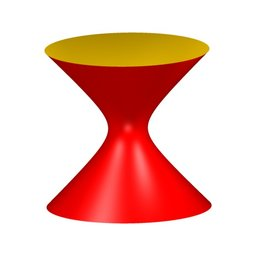
\includegraphics[width=1.2cm]{./../../common/images/A1pm_2}
        \end{tabular}
        &
        $\leftarrow$
        &
        \begin{tabular}{@{}c@{}}
          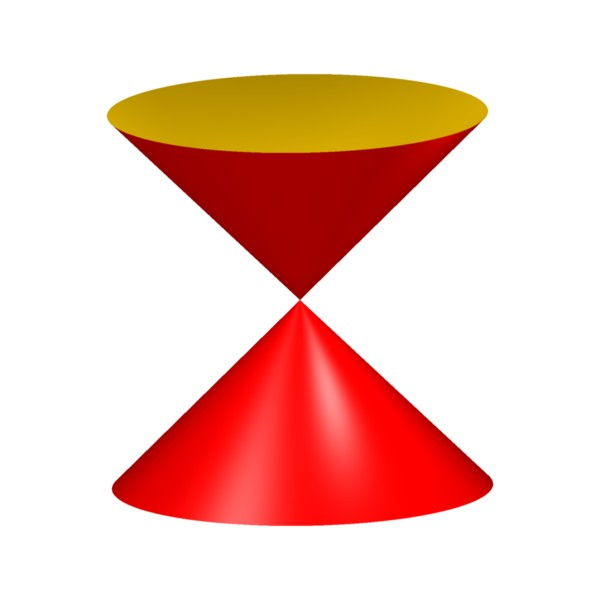
\includegraphics[width=1.2cm]{./../../common/images/A1pm_1} 
        \end{tabular}
        &
        $\rightarrow$
        &
        \begin{tabular}{@{}c@{}}
          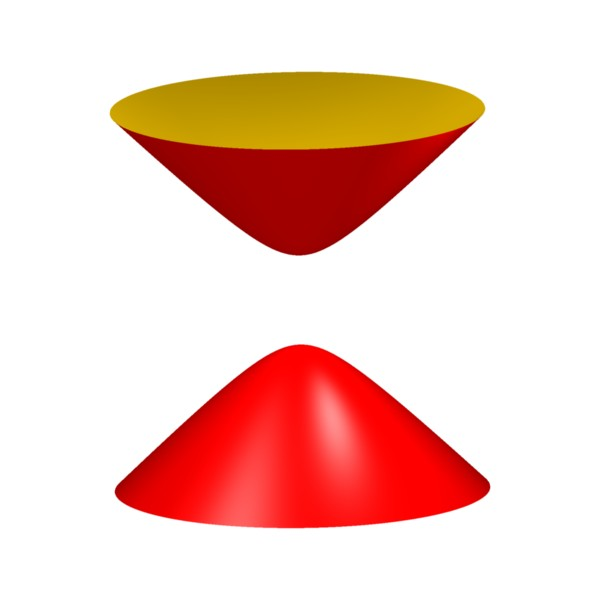
\includegraphics[width=1.2cm]{./../../common/images/A1pm_0}
        \end{tabular}
      \end{tabular}
    \end{center}
   A surface of degree $2$ cannot have more than one singularity, i.e.\ $\mu(2)=1$.
\end{surferPage}
